% Options for packages loaded elsewhere
\PassOptionsToPackage{unicode}{hyperref}
\PassOptionsToPackage{hyphens}{url}
%
\documentclass[
]{article}
\usepackage{amsmath,amssymb}
\usepackage{lmodern}
\usepackage{iftex}
\ifPDFTeX
  \usepackage[T1]{fontenc}
  \usepackage[utf8]{inputenc}
  \usepackage{textcomp} % provide euro and other symbols
\else % if luatex or xetex
  \usepackage{unicode-math}
  \defaultfontfeatures{Scale=MatchLowercase}
  \defaultfontfeatures[\rmfamily]{Ligatures=TeX,Scale=1}
\fi
% Use upquote if available, for straight quotes in verbatim environments
\IfFileExists{upquote.sty}{\usepackage{upquote}}{}
\IfFileExists{microtype.sty}{% use microtype if available
  \usepackage[]{microtype}
  \UseMicrotypeSet[protrusion]{basicmath} % disable protrusion for tt fonts
}{}
\makeatletter
\@ifundefined{KOMAClassName}{% if non-KOMA class
  \IfFileExists{parskip.sty}{%
    \usepackage{parskip}
  }{% else
    \setlength{\parindent}{0pt}
    \setlength{\parskip}{6pt plus 2pt minus 1pt}}
}{% if KOMA class
  \KOMAoptions{parskip=half}}
\makeatother
\usepackage{xcolor}
\IfFileExists{xurl.sty}{\usepackage{xurl}}{} % add URL line breaks if available
\IfFileExists{bookmark.sty}{\usepackage{bookmark}}{\usepackage{hyperref}}
\hypersetup{
  pdftitle={Untitled},
  hidelinks,
  pdfcreator={LaTeX via pandoc}}
\urlstyle{same} % disable monospaced font for URLs
\usepackage[margin=1in]{geometry}
\usepackage{color}
\usepackage{fancyvrb}
\newcommand{\VerbBar}{|}
\newcommand{\VERB}{\Verb[commandchars=\\\{\}]}
\DefineVerbatimEnvironment{Highlighting}{Verbatim}{commandchars=\\\{\}}
% Add ',fontsize=\small' for more characters per line
\usepackage{framed}
\definecolor{shadecolor}{RGB}{248,248,248}
\newenvironment{Shaded}{\begin{snugshade}}{\end{snugshade}}
\newcommand{\AlertTok}[1]{\textcolor[rgb]{0.94,0.16,0.16}{#1}}
\newcommand{\AnnotationTok}[1]{\textcolor[rgb]{0.56,0.35,0.01}{\textbf{\textit{#1}}}}
\newcommand{\AttributeTok}[1]{\textcolor[rgb]{0.77,0.63,0.00}{#1}}
\newcommand{\BaseNTok}[1]{\textcolor[rgb]{0.00,0.00,0.81}{#1}}
\newcommand{\BuiltInTok}[1]{#1}
\newcommand{\CharTok}[1]{\textcolor[rgb]{0.31,0.60,0.02}{#1}}
\newcommand{\CommentTok}[1]{\textcolor[rgb]{0.56,0.35,0.01}{\textit{#1}}}
\newcommand{\CommentVarTok}[1]{\textcolor[rgb]{0.56,0.35,0.01}{\textbf{\textit{#1}}}}
\newcommand{\ConstantTok}[1]{\textcolor[rgb]{0.00,0.00,0.00}{#1}}
\newcommand{\ControlFlowTok}[1]{\textcolor[rgb]{0.13,0.29,0.53}{\textbf{#1}}}
\newcommand{\DataTypeTok}[1]{\textcolor[rgb]{0.13,0.29,0.53}{#1}}
\newcommand{\DecValTok}[1]{\textcolor[rgb]{0.00,0.00,0.81}{#1}}
\newcommand{\DocumentationTok}[1]{\textcolor[rgb]{0.56,0.35,0.01}{\textbf{\textit{#1}}}}
\newcommand{\ErrorTok}[1]{\textcolor[rgb]{0.64,0.00,0.00}{\textbf{#1}}}
\newcommand{\ExtensionTok}[1]{#1}
\newcommand{\FloatTok}[1]{\textcolor[rgb]{0.00,0.00,0.81}{#1}}
\newcommand{\FunctionTok}[1]{\textcolor[rgb]{0.00,0.00,0.00}{#1}}
\newcommand{\ImportTok}[1]{#1}
\newcommand{\InformationTok}[1]{\textcolor[rgb]{0.56,0.35,0.01}{\textbf{\textit{#1}}}}
\newcommand{\KeywordTok}[1]{\textcolor[rgb]{0.13,0.29,0.53}{\textbf{#1}}}
\newcommand{\NormalTok}[1]{#1}
\newcommand{\OperatorTok}[1]{\textcolor[rgb]{0.81,0.36,0.00}{\textbf{#1}}}
\newcommand{\OtherTok}[1]{\textcolor[rgb]{0.56,0.35,0.01}{#1}}
\newcommand{\PreprocessorTok}[1]{\textcolor[rgb]{0.56,0.35,0.01}{\textit{#1}}}
\newcommand{\RegionMarkerTok}[1]{#1}
\newcommand{\SpecialCharTok}[1]{\textcolor[rgb]{0.00,0.00,0.00}{#1}}
\newcommand{\SpecialStringTok}[1]{\textcolor[rgb]{0.31,0.60,0.02}{#1}}
\newcommand{\StringTok}[1]{\textcolor[rgb]{0.31,0.60,0.02}{#1}}
\newcommand{\VariableTok}[1]{\textcolor[rgb]{0.00,0.00,0.00}{#1}}
\newcommand{\VerbatimStringTok}[1]{\textcolor[rgb]{0.31,0.60,0.02}{#1}}
\newcommand{\WarningTok}[1]{\textcolor[rgb]{0.56,0.35,0.01}{\textbf{\textit{#1}}}}
\usepackage{longtable,booktabs,array}
\usepackage{calc} % for calculating minipage widths
% Correct order of tables after \paragraph or \subparagraph
\usepackage{etoolbox}
\makeatletter
\patchcmd\longtable{\par}{\if@noskipsec\mbox{}\fi\par}{}{}
\makeatother
% Allow footnotes in longtable head/foot
\IfFileExists{footnotehyper.sty}{\usepackage{footnotehyper}}{\usepackage{footnote}}
\makesavenoteenv{longtable}
\usepackage{graphicx}
\makeatletter
\def\maxwidth{\ifdim\Gin@nat@width>\linewidth\linewidth\else\Gin@nat@width\fi}
\def\maxheight{\ifdim\Gin@nat@height>\textheight\textheight\else\Gin@nat@height\fi}
\makeatother
% Scale images if necessary, so that they will not overflow the page
% margins by default, and it is still possible to overwrite the defaults
% using explicit options in \includegraphics[width, height, ...]{}
\setkeys{Gin}{width=\maxwidth,height=\maxheight,keepaspectratio}
% Set default figure placement to htbp
\makeatletter
\def\fps@figure{htbp}
\makeatother
\setlength{\emergencystretch}{3em} % prevent overfull lines
\providecommand{\tightlist}{%
  \setlength{\itemsep}{0pt}\setlength{\parskip}{0pt}}
\setcounter{secnumdepth}{5}
\usepackage{subfig}
\ifLuaTeX
  \usepackage{selnolig}  % disable illegal ligatures
\fi

\title{Untitled}
\author{}
\date{\vspace{-2.5em}2022-06-11}

\begin{document}
\maketitle

{
\setcounter{tocdepth}{2}
\tableofcontents
}
\hypertarget{r-markdown}{%
\subsection{R Markdown}\label{r-markdown}}

\begin{Shaded}
\begin{Highlighting}[]
\NormalTok{EViews\textgreater{} wfcreate(wf=sagiru,page=mati) q 2000 2025}
\NormalTok{+ for \%y page1 page2 page3  }
\NormalTok{+ pagecreate(page=\{\%y\}) q 2000 2025}
\NormalTok{+ next}
\NormalTok{+ \%pagelist=@pagelist}
\NormalTok{+ \textquotesingle{}open mychunk}
\NormalTok{+ for \%y \{\%pagelist\}}
\NormalTok{+ pageselect \{\%y\}}
\NormalTok{+ delete gra*}
\NormalTok{+ genr y=@cumsum(nrnd)}
\NormalTok{+ genr x=@cumsum(nrnd)}
\NormalTok{+ genr z=@cumsum(nrnd)}
\NormalTok{+ genr date=@date}
\NormalTok{+                      graph grap1.dot z  }
\NormalTok{+                            graph grap2.bar y }
\NormalTok{+                            graph grap3.area x  }
\NormalTok{+    freeze(grap,mode=overwrite) x.line}
\NormalTok{+ equation ols.ls y c x}
\NormalTok{+ freeze(tab) ols}
\NormalTok{+ next}
\NormalTok{+ wfsave mychunk}
\end{Highlighting}
\end{Shaded}

\begin{figure}[h]

{\centering \subfloat[Page 1 Figure 1\label{fig:mychunk-1}]{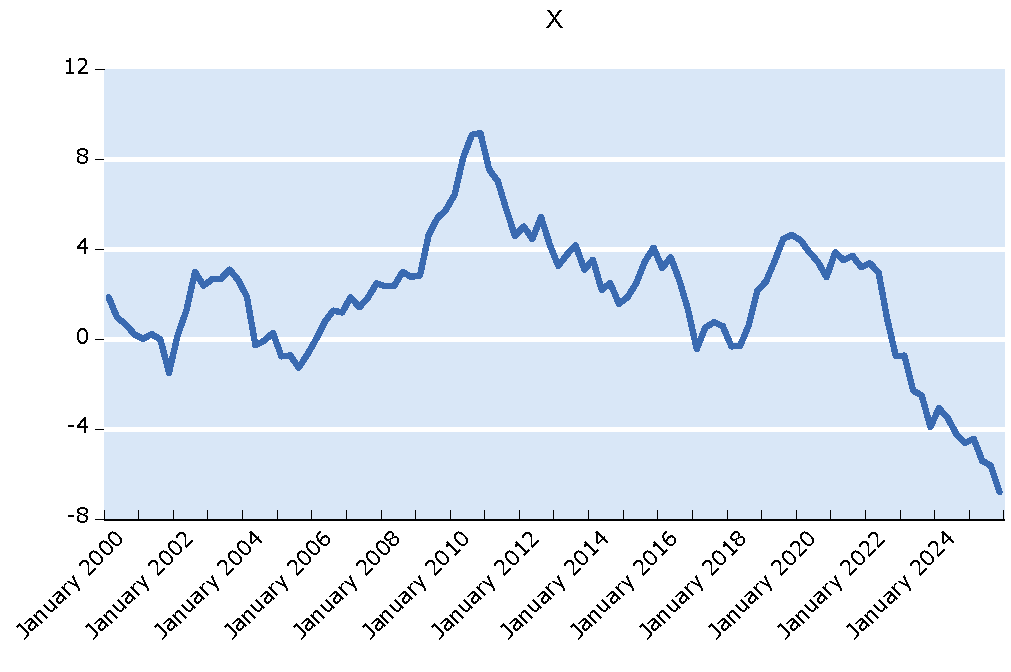
\includegraphics[width=0.25\textwidth]{test_engEviews_files/figure-latex//mychunk-mati-grap} }\subfloat[Page 1 Figure 2\label{fig:mychunk-2}]{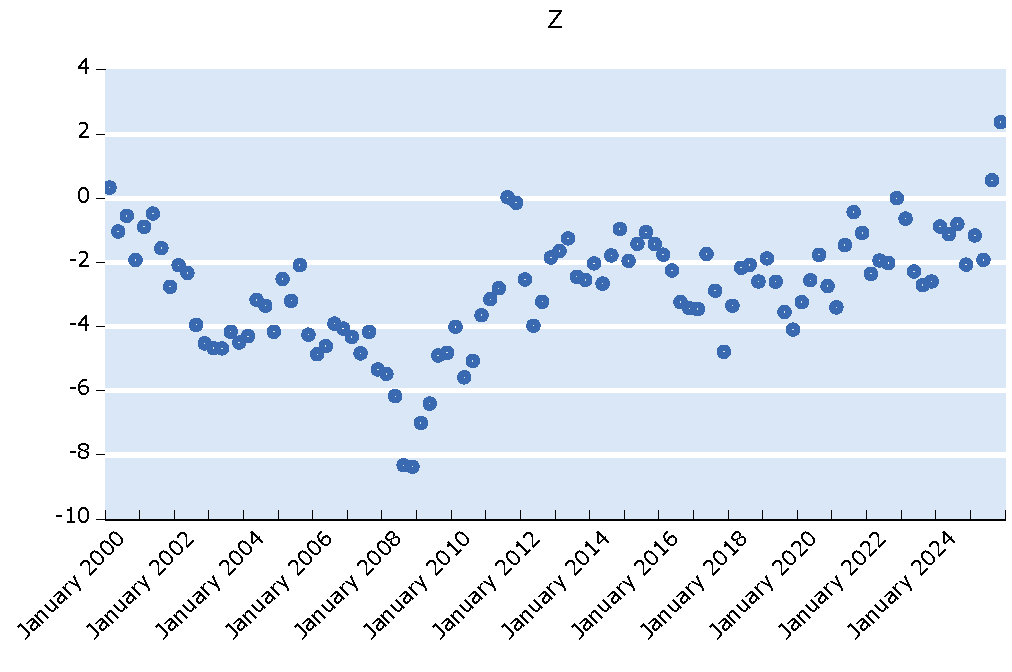
\includegraphics[width=0.25\textwidth]{test_engEviews_files/figure-latex//mychunk-mati-grap1} }\subfloat[Page 1 Figure 3\label{fig:mychunk-3}]{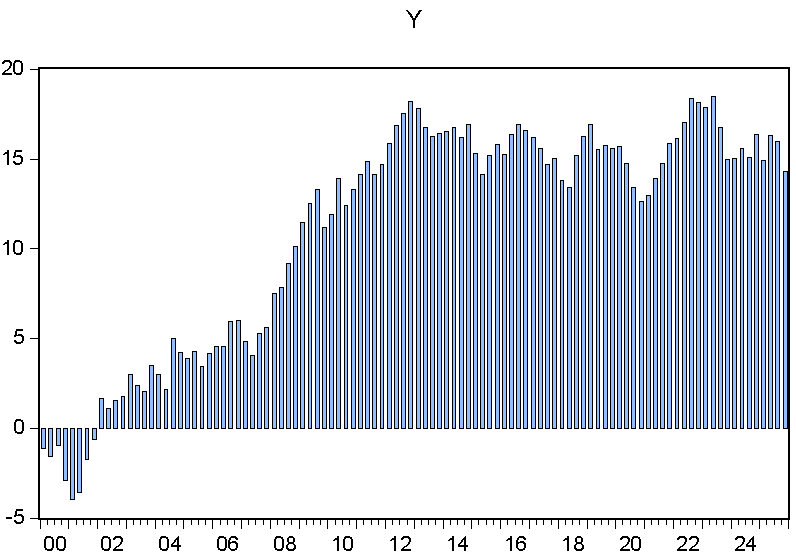
\includegraphics[width=0.25\textwidth]{test_engEviews_files/figure-latex//mychunk-mati-grap2} }\subfloat[Page 1 Figure 4\label{fig:mychunk-4}]{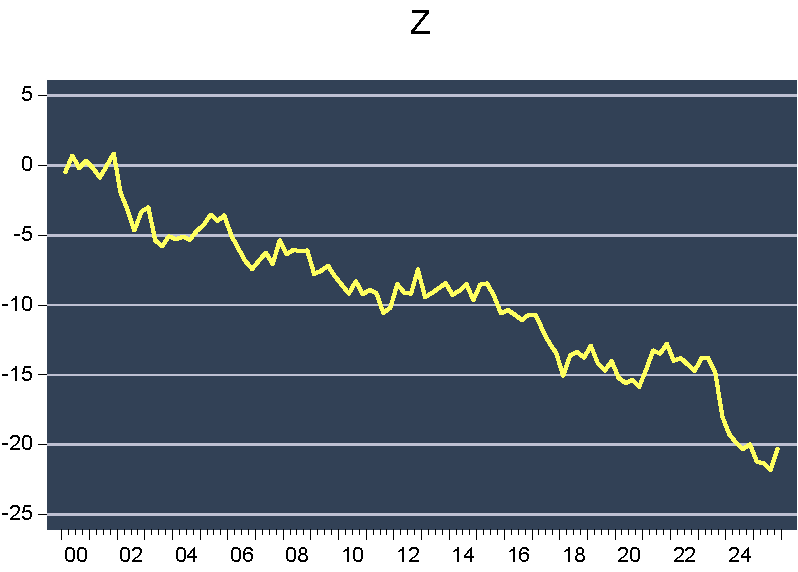
\includegraphics[width=0.25\textwidth]{test_engEviews_files/figure-latex//mychunk-mati-grap3} }\newline\subfloat[Page 2 Figure 1\label{fig:mychunk-5}]{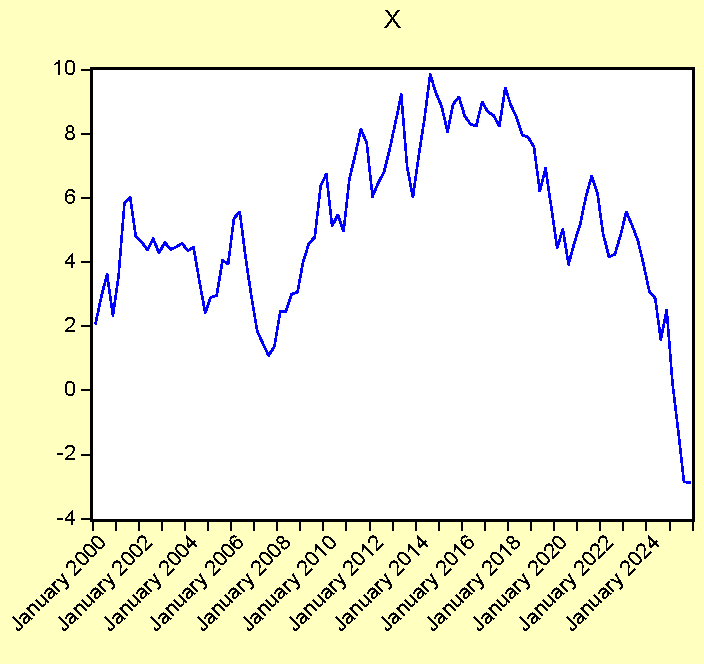
\includegraphics[width=0.25\textwidth]{test_engEviews_files/figure-latex//mychunk-page1-grap} }\subfloat[Page 2 Figure 2\label{fig:mychunk-6}]{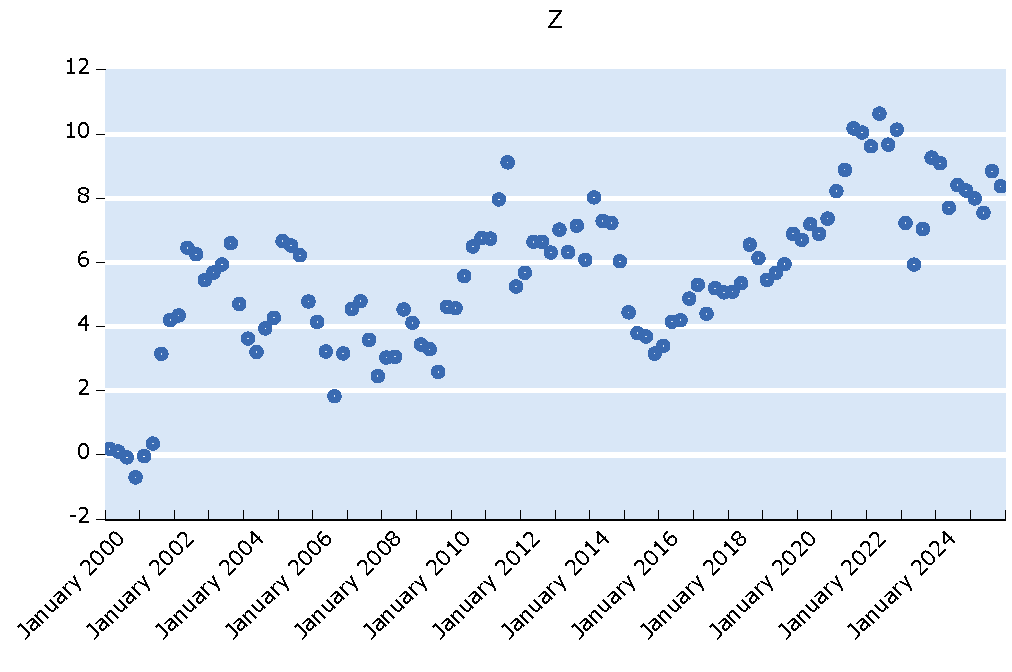
\includegraphics[width=0.25\textwidth]{test_engEviews_files/figure-latex//mychunk-page1-grap1} }\subfloat[Page 2 Figure 3\label{fig:mychunk-7}]{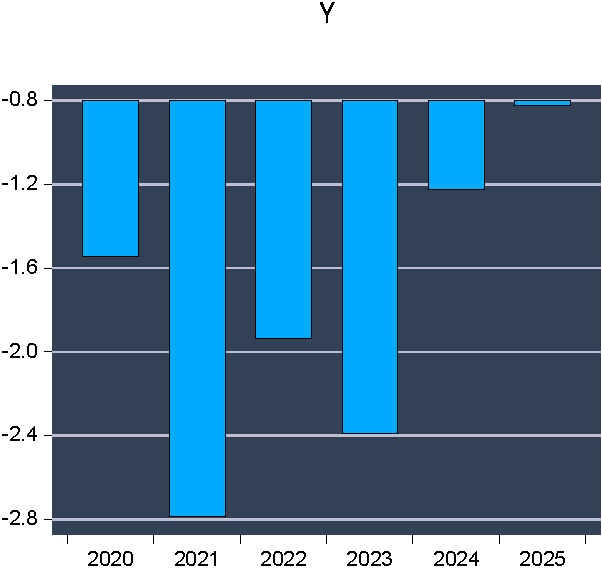
\includegraphics[width=0.25\textwidth]{test_engEviews_files/figure-latex//mychunk-page1-grap2} }\subfloat[Page 2 Figure 4\label{fig:mychunk-8}]{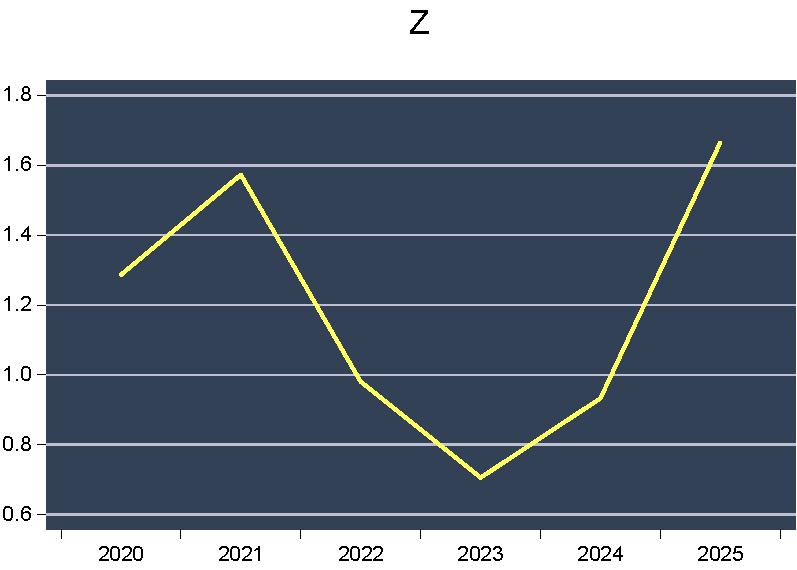
\includegraphics[width=0.25\textwidth]{test_engEviews_files/figure-latex//mychunk-page1-grap3} }\newline\subfloat[Page 3 Figure 1\label{fig:mychunk-9}]{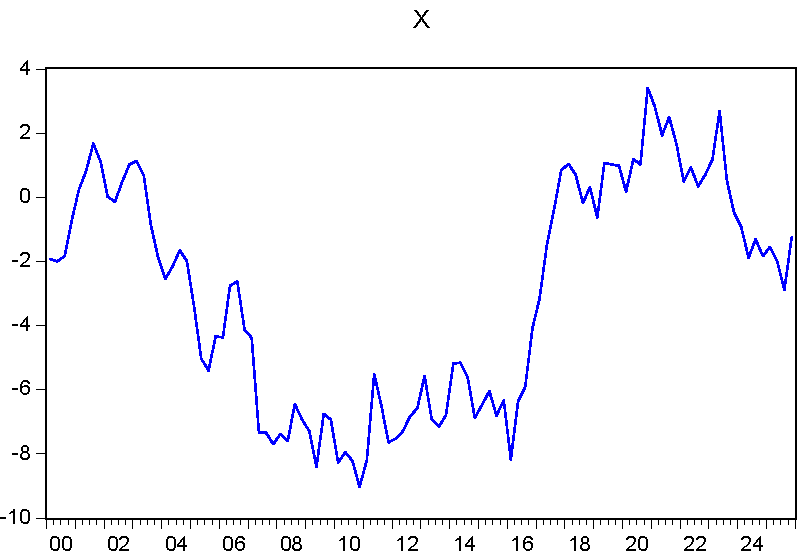
\includegraphics[width=0.25\textwidth]{test_engEviews_files/figure-latex//mychunk-page2-grap} }\subfloat[Page 3 Figure 2\label{fig:mychunk-10}]{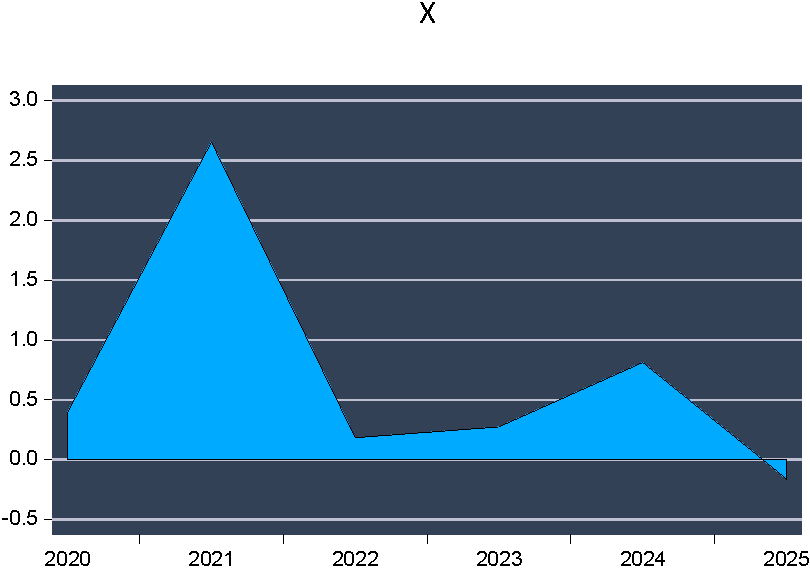
\includegraphics[width=0.25\textwidth]{test_engEviews_files/figure-latex//mychunk-page2-grap1} }\subfloat[Page 3 Figure 3\label{fig:mychunk-11}]{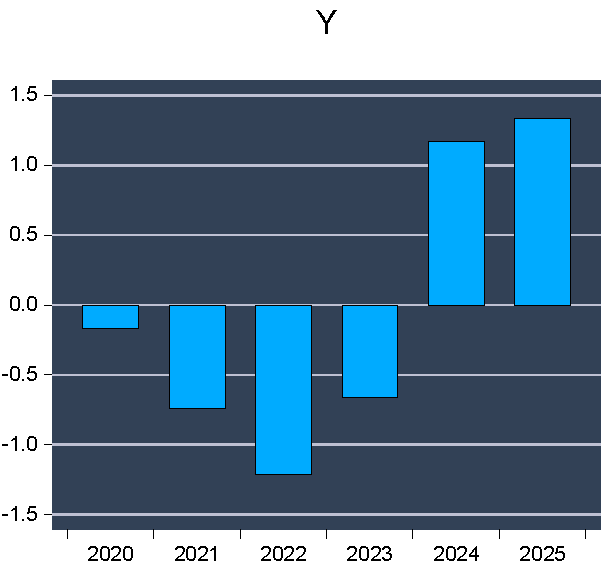
\includegraphics[width=0.25\textwidth]{test_engEviews_files/figure-latex//mychunk-page2-grap2} }\subfloat[Page 3 Figure 4\label{fig:mychunk-12}]{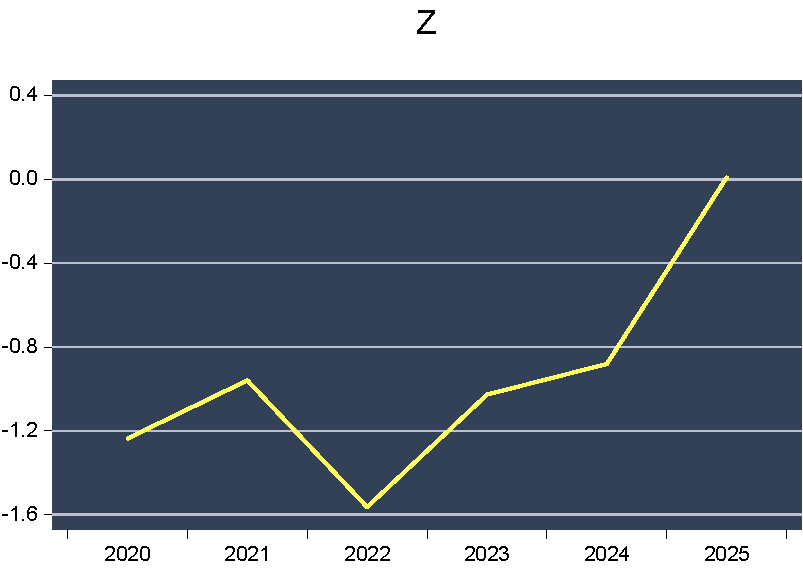
\includegraphics[width=0.25\textwidth]{test_engEviews_files/figure-latex//mychunk-page2-grap3} }\newline\subfloat[Page 4 Figure 1\label{fig:mychunk-13}]{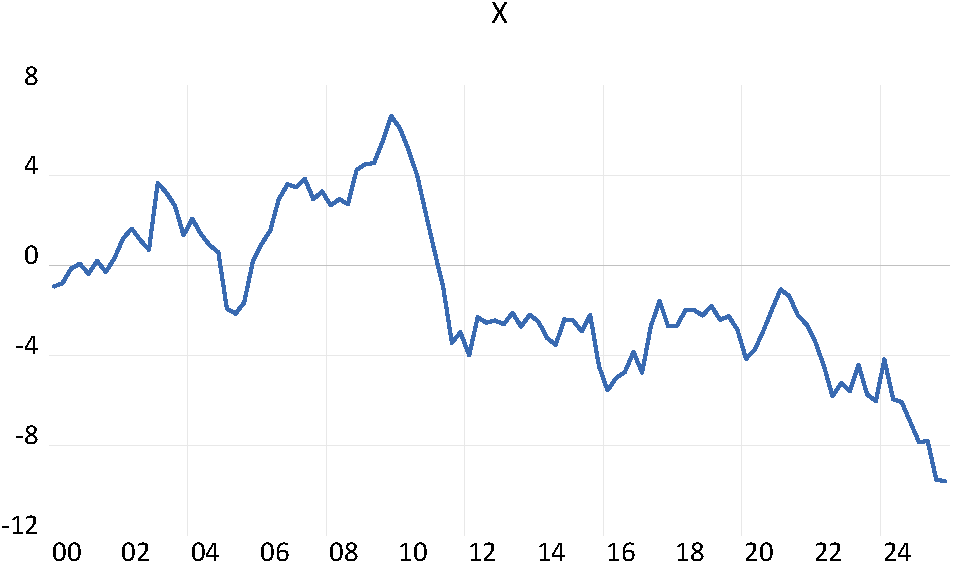
\includegraphics[width=0.25\textwidth]{test_engEviews_files/figure-latex//mychunk-page3-grap} }\subfloat[Page 4 Figure 2\label{fig:mychunk-14}]{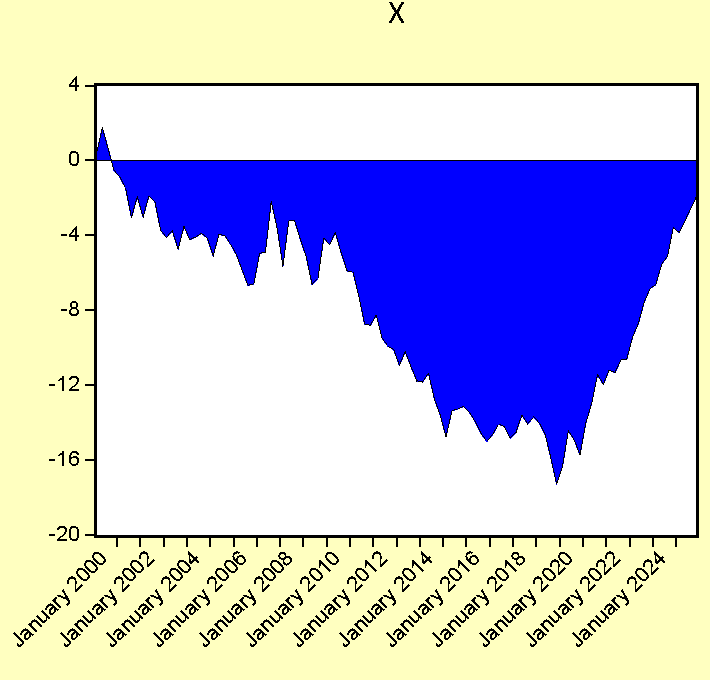
\includegraphics[width=0.25\textwidth]{test_engEviews_files/figure-latex//mychunk-page3-grap1} }\subfloat[Page 4 Figure 3\label{fig:mychunk-15}]{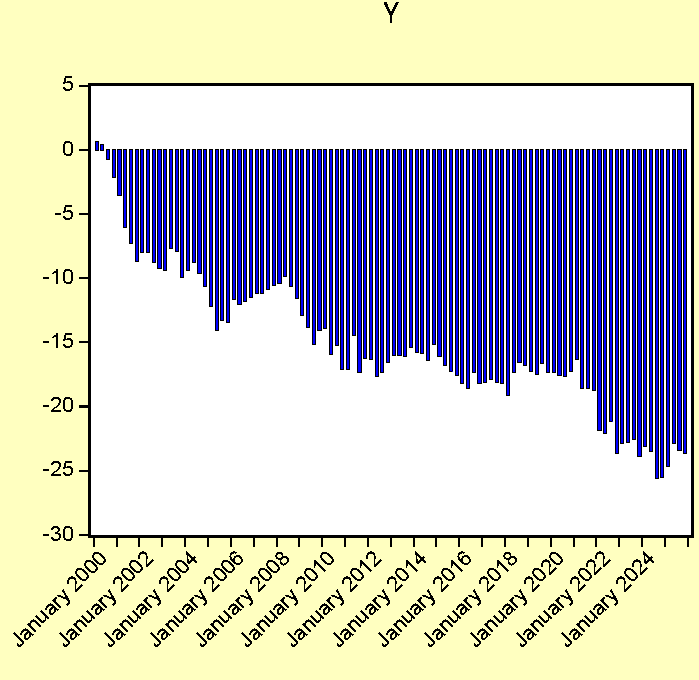
\includegraphics[width=0.25\textwidth]{test_engEviews_files/figure-latex//mychunk-page3-grap2} }\subfloat[Page 4 Figure 4\label{fig:mychunk-16}]{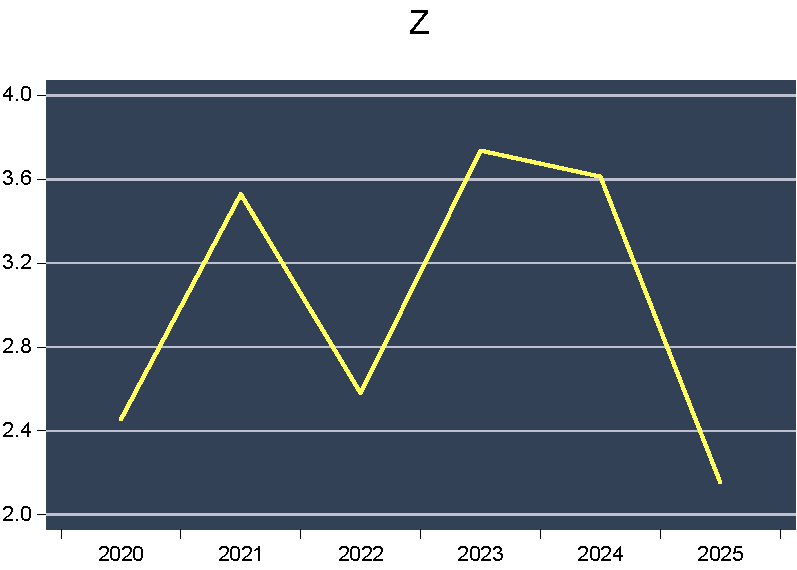
\includegraphics[width=0.25\textwidth]{test_engEviews_files/figure-latex//mychunk-page3-grap3} }

}

\caption{somefigure}\label{fig:mychunk}
\end{figure}

\begin{verbatim}
## NULL
\end{verbatim}

\begin{verbatim}
## NULL
\end{verbatim}

\begin{verbatim}
## NULL
\end{verbatim}

\begin{verbatim}
##         date         x           y         z
## 1 2000-01-01 0.3581780 -0.28670142 -1.252282
## 2 2000-04-01 0.7225110 -0.15422686 -2.374090
## 3 2000-07-01 0.6264368 -0.01970857 -1.191394
## 4 2000-10-01 1.5622026  1.71801486 -1.307479
## 5 2001-01-01 2.1920427  1.57692462 -1.047143
## 6 2001-04-01 1.2774845  1.83442578 -2.118365
\end{verbatim}

\hypertarget{r-plots}{%
\section{R plots}\label{r-plots}}

\begin{verbatim}
## NULL
\end{verbatim}

\begin{verbatim}
## [1] "asis"
\end{verbatim}

\begin{figure}[h]

{\centering 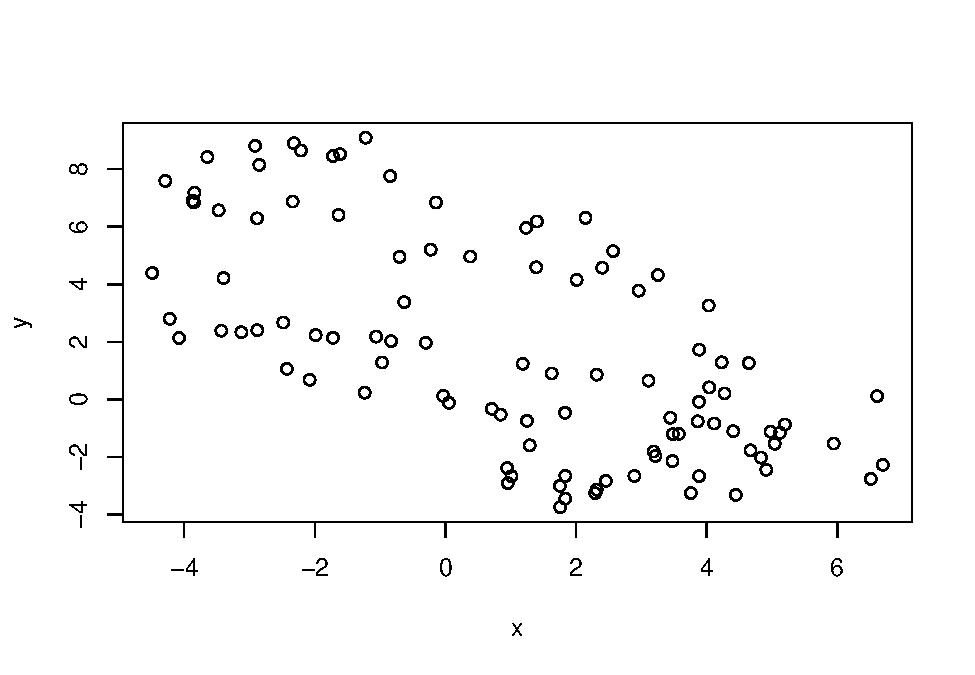
\includegraphics[width=0.45\textwidth]{test_engEviews_files/figure-latex/labe-1} 

}

\caption{another fig}\label{fig:labe}
\end{figure}

\begin{center}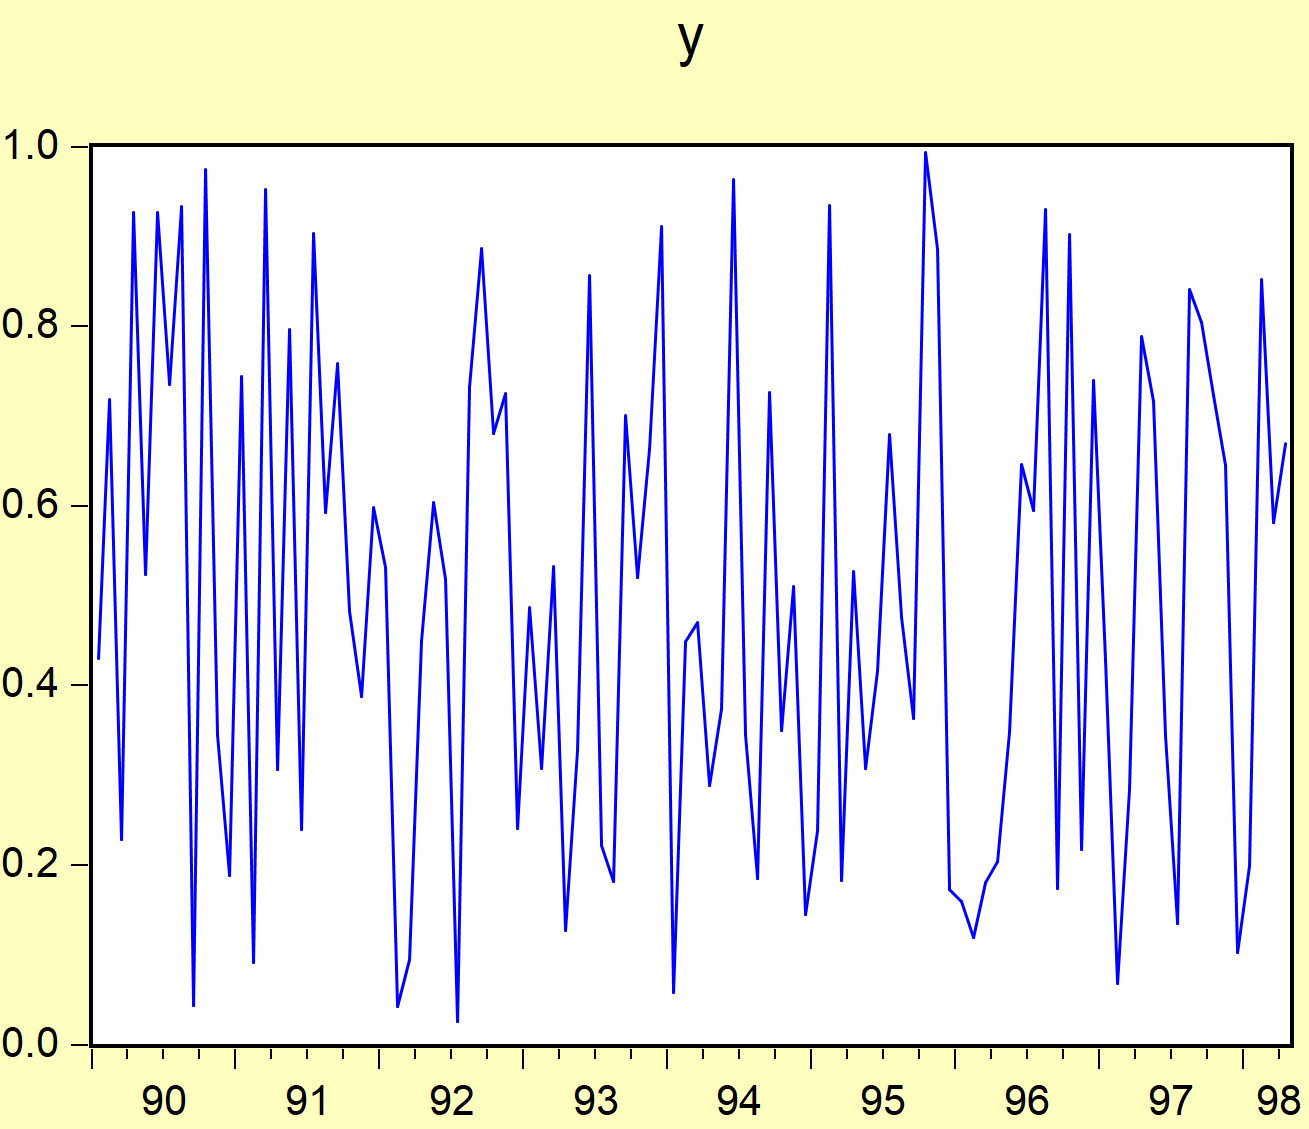
\includegraphics[width=0.45\textwidth]{test_engEviews_files/figure-latex//eview-graph-y} \end{center}

\begin{center}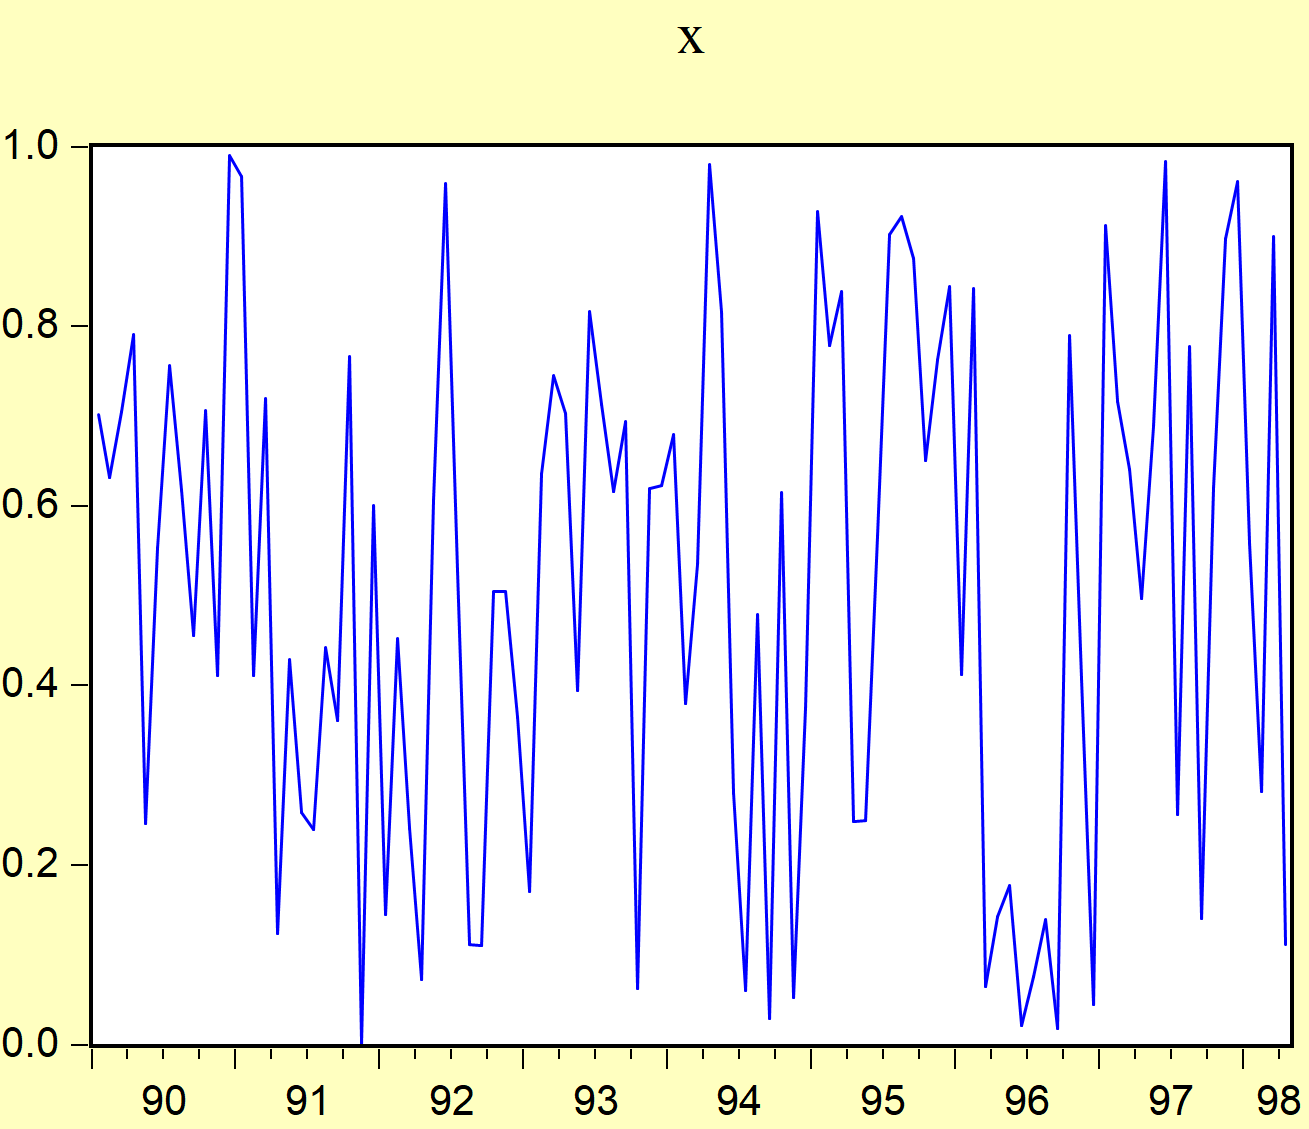
\includegraphics[width=0.45\textwidth]{test_engEviews_files/figure-latex//eview-graph-x} \end{center}

\begin{verbatim}
##         date          x           y          z
## 1 2001-01-01 -0.2459328  0.27925204  0.2001161
## 2 2001-01-02 -0.1874220 -0.29029595  0.1853385
## 3 2001-01-03  1.6102392  1.59160047  3.2885122
## 4 2001-01-04  2.1732303  0.08786238  2.8418956
## 5 2001-01-05  1.4192666 -0.13008483 -0.2284603
## 6 2001-01-06  1.1725949  0.09164000 -1.6514512
\end{verbatim}

\begin{center}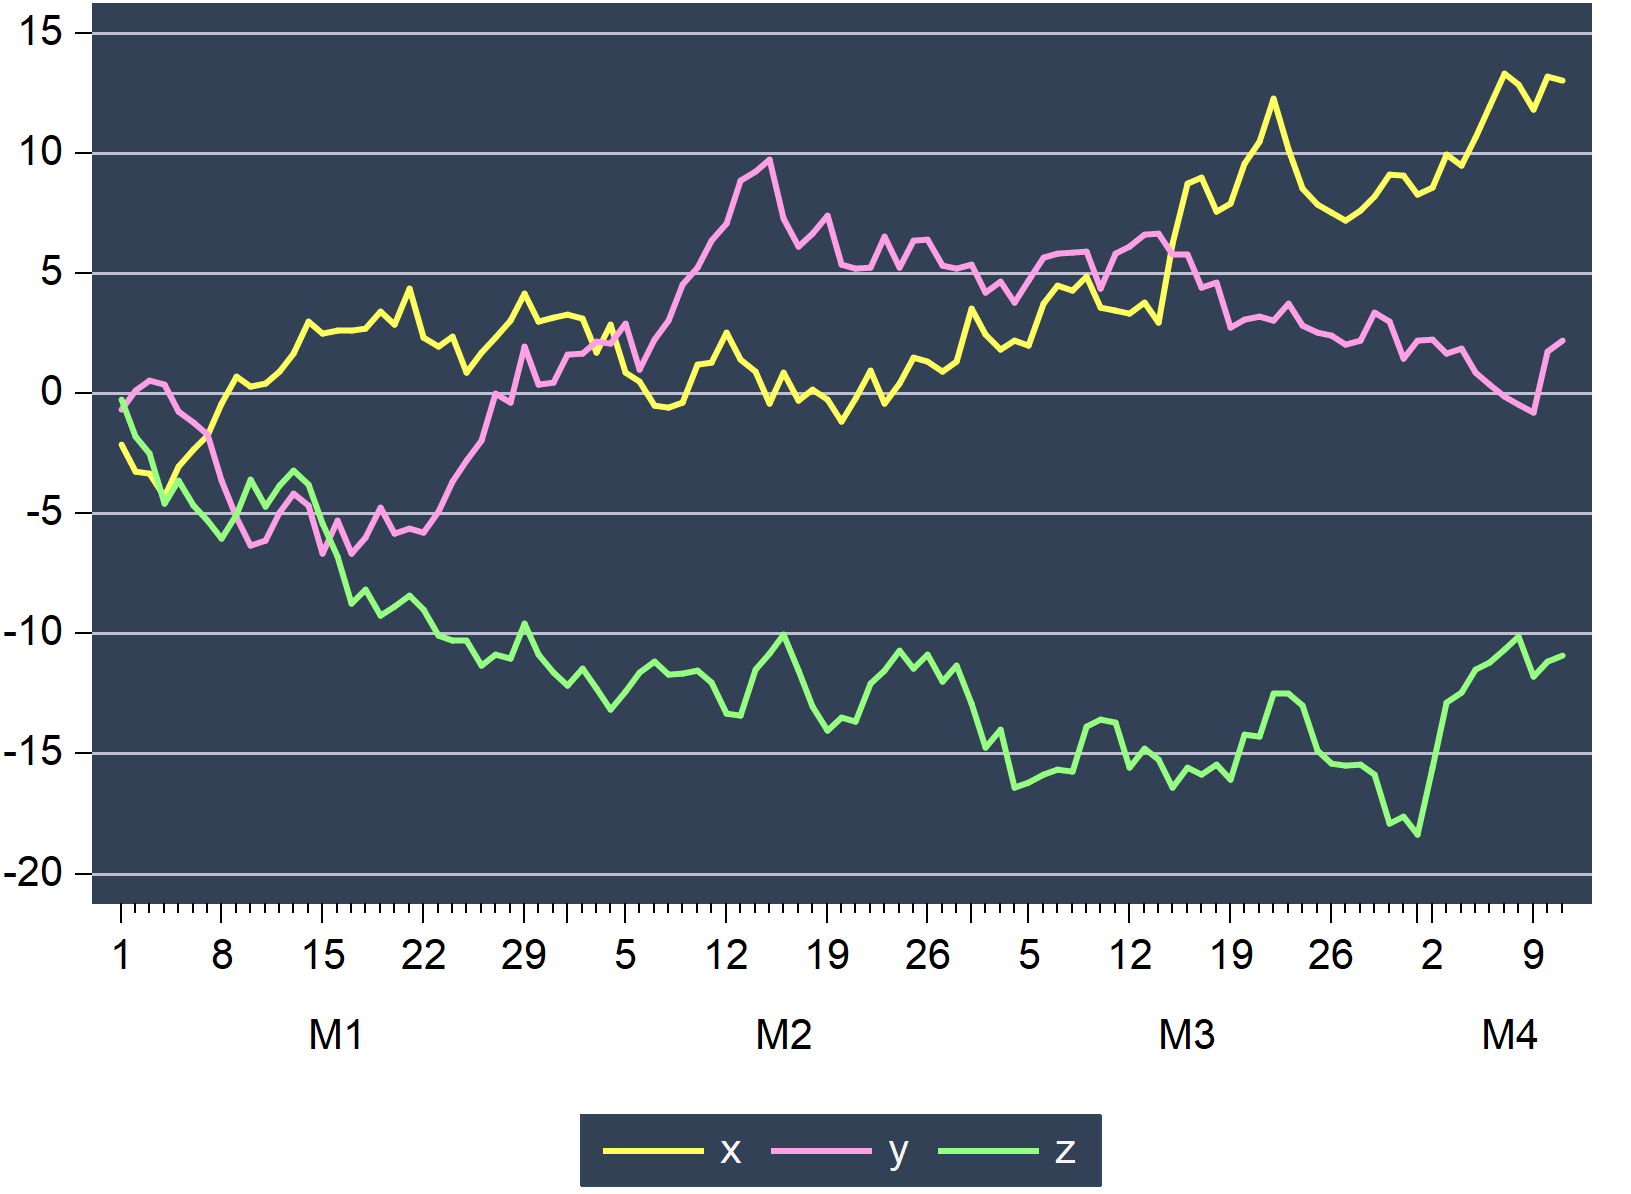
\includegraphics[width=0.45\textwidth]{test_engEviews_files/figure-latex//rwalk-xyz} \end{center}

\end{document}
